%%%%%%%%%%%%%%%%%%%%%%%%%%%%%%%%%%%%%%%%%
% Arsclassica Article
% LaTeX Template
% Version 1.1 (10/6/14)
%
% This template has been downloaded from:
% http://www.LaTeXTemplates.com
%
% Original author:
% Lorenzo Pantieri (http://www.lorenzopantieri.net) with extensive modifications by:
% Vel (vel@latextemplates.com)
% Johan Bos (johan.bos@rug.nl)
%
% License:
% CC BY-NC-SA 3.0 (http://creativecommons.org/licenses/by-nc-sa/3.0/)
%
%%%%%%%%%%%%%%%%%%%%%%%%%%%%%%%%%%%%%%%%%

%----------------------------------------------------------------------------------------
%	PACKAGES AND OTHER DOCUMENT CONFIGURATIONS
%----------------------------------------------------------------------------------------

\documentclass[
10pt, % Main document font size
a4paper, % Paper type, use 'letterpaper' for US Letter paper
oneside, % One page layout (no page indentation)
%twoside, % Two page layout (page indentation for binding and different headers)
headinclude,footinclude, % Extra spacing for the header and footer
%BCOR5mm, % Binding correction
] {book}% {scrartcl}

%%%%%%%%%%%%%%%%%%%%%%%%%%%%%%%%%%%%%%%%%
% Arsclassica Article
% Structure Specification File
%
% This file has been downloaded from:
% http://www.LaTeXTemplates.com
%
% Original author:
% Lorenzo Pantieri (http://www.lorenzopantieri.net) with extensive modifications by:
% Vel (vel@latextemplates.com)
%
% License:
% CC BY-NC-SA 3.0 (http://creativecommons.org/licenses/by-nc-sa/3.0/)
%
%%%%%%%%%%%%%%%%%%%%%%%%%%%%%%%%%%%%%%%%%

%----------------------------------------------------------------------------------------
%	REQUIRED PACKAGES
%----------------------------------------------------------------------------------------

\usepackage[
%nochapters, % Turn off chapters since this is an article        
beramono, % Use the Bera Mono font for monospaced text (\texttt)
eulermath,% Use the Euler font for mathematics
pdfspacing, % Makes use of pdftex letter spacing capabilities via the microtype package
dottedtoc % Dotted lines leading to the page numbers in the table of contents
]{classicthesis} % The layout is based on the Classic Thesis style


\usepackage{arsclassica} % Modifies the Classic Thesis package

\usepackage[T1]{fontenc} % Use 8-bit encoding that has 256 glyphs

\usepackage[utf8]{inputenc} % Required for including letters with accents

\usepackage{graphicx} % Required for including images

\usepackage{enumitem} % Required for manipulating the whitespace between and within lists

\usepackage{lipsum} % Used for inserting dummy 'Lorem ipsum' text into the template

\usepackage{subfig} % Required for creating figures with multiple parts (subfigures)

\usepackage{amsmath,amssymb,amsthm} % For including math equations, theorems, symbols, etc

\usepackage{varioref} % More descriptive referencing
\usepackage{color}
\usepackage{listings}
\usepackage{setspace}
\usepackage{lscape}
\usepackage[authoryear]{natbib}

%----------------------------------------------------------------------------------------
%	DUTCH SUPPORT
%----------------------------------------------------------------------------------------

%\usepackage[dutch]{babel}    % comment out if you write your thesis in Dutch


%----------------------------------------------------------------------------------------
%	THEOREM STYLES
%---------------------------------------------------------------------------------------

\theoremstyle{definition} % Define theorem styles here based on the definition style (used for definitions and examples)
\newtheorem{definition}{Definition}

\theoremstyle{plain} % Define theorem styles here based on the plain style (used for theorems, lemmas, propositions)
\newtheorem{theorem}{Theorem}

\theoremstyle{remark} % Define theorem styles here based on the remark style (used for remarks and notes)

%----------------------------------------------------------------------------------------
%	HYPERLINKS
%---------------------------------------------------------------------------------------

\hypersetup{
%draft, % Uncomment to remove all links (useful for printing in black and white)
colorlinks=true, breaklinks=true, % bookmarks=true,
bookmarksnumbered,
urlcolor=webbrown, linkcolor=RoyalBlue, citecolor=webgreen, % Link colors
pdftitle={}, % PDF title
pdfauthor={\textcopyright}, % PDF Author
pdfsubject={}, % PDF Subject
pdfkeywords={}, % PDF Keywords
pdfcreator={pdfLaTeX}, % PDF Creator
plainpages=false,
pdfproducer={LaTeX with hyperref and ClassicThesis} % PDF producer
}


\renewcommand{\lstlistingname}{Python code}% Listing -> Python
\renewcommand{\lstlistlistingname}{List of \lstlistingname}% List of Listings -> List of Python
\definecolor{Code}{rgb}{0,0,0}
\definecolor{Decorators}{rgb}{0.5,0.5,0.5}
\definecolor{Numbers}{rgb}{0.5,0,0}
\definecolor{MatchingBrackets}{rgb}{0.25,0.5,0.5}
\definecolor{Keywords}{rgb}{0,0,1}
\definecolor{self}{rgb}{0,0,0}
\definecolor{Strings}{rgb}{0,0.63,0}
\definecolor{Comments}{rgb}{0,0.63,1}
\definecolor{Backquotes}{rgb}{0,0,0}
\definecolor{Classname}{rgb}{0,0,0}
\definecolor{FunctionName}{rgb}{0,0,0}
\definecolor{Operators}{rgb}{0,0,0}
\definecolor{Background}{rgb}{0.98,0.98,0.98}




 
\lstdefinestyle{mystyle}{
numbers=left,
numberstyle=\footnotesize,
numbersep=1em,
xleftmargin=1em,
framextopmargin=10em,
framexbottommargin=2em,
showspaces=false,
showtabs=false,
showstringspaces=false,
frame=l,
tabsize=4,
% Basic
basicstyle=\ttfamily\small\setstretch{1},
backgroundcolor=\color{Background},
language=Python,
% Comments
commentstyle=\color{Comments}\slshape,
% Strings
stringstyle=\color{Strings},
morecomment=[s][\color{Strings}]{"""}{"""},
morecomment=[s][\color{Strings}]{'''}{'''},
% keywords
morekeywords={import,from,class,def,for,while,if,is,in,elif,else,not,and,or,print,break,continue,return,True,False,None,access,as,,del,except,exec,finally,global,import,lambda,pass,print,raise,try,assert},
keywordstyle={\color{Keywords}\bfseries},
% additional keywords
morekeywords={[2]@invariant},
keywordstyle={[2]\color{Decorators}\slshape},
emph={self},
emphstyle={\color{self}\slshape},
captionpos=b, 
}
 
\lstset{style=mystyle}

\def\vl{\\[9pt]}
 % Include the structure.tex file which specified the document structure and layout

\usepackage{booktabs}
\usepackage{natbib}
\usepackage{url}

%----------------------------------------------------------------------------------------
%	HYPHENATION
%----------------------------------------------------------------------------------------

\hyphenation{Fortran hy-phen-ation} % Specify custom hyphenation points in words with dashes where you would like hyphenation to occur, or alternatively, don't put any dashes in a word to stop hyphenation altogether



%----------------------------------------------------------------------------------------
%	TITLE AND AUTHOR(S)
%----------------------------------------------------------------------------------------

\title{\normalfont\spacedallcaps{title}} % The article title

\author{\spacedlowsmallcaps{author}} % The article author(s) - author affiliations need to be specified in the AUTHOR AFFILIATIONS block

\date{} % An optional date to appear under the author(s)

%----------------------------------------------------------------------------------------

\begin{document}

%----------------------------------------------------------------------------------------
%	HEADERS
%----------------------------------------------------------------------------------------

%\renewcommand{\chaptermark}[1]{\markright{\spacedlowsmallcaps{#1}}} % The header for all pages (oneside) or for even pages (twoside)
%\renewcommand{\subsectionmark}[1]{\markright{\thesubsection~#1}} % Uncomment when using the twoside option - this modifies the header on odd pages
%\lehead{\mbox{\llap{\small\thepage\kern1em\color{halfgray} \vline}\color{halfgray}\hspace{0.5em}\rightmark\hfil}} % The header style

\pagestyle{scrheadings} % Enable the headers specified in this block


%----------------------------------------------------------------------------------------
%	TITLE PAGE
%----------------------------------------------------------------------------------------

\hypersetup{pageanchor=false}
\begin{titlepage}
\thispagestyle{empty}
\begin{figure}[h!] %  figure placement: here, top, bottom, or page

\includegraphics[width=4in]{ruglogo} 
\end{figure}

\begin{center}
\vspace{30 mm}
\begingroup \linespread{1,75} \selectfont 
\textsc{\LARGE Movie Review Mastery}\\
\textsc{\Large Automatic sentiment analysis for movie reviews, based on general and movie-specific textual features}\\[1,5cm]
\endgroup

Tom Kosse\\[2,5cm]

\end{center}
\vfill
\textbf{Bachelor thesis}\\  %\textbf{Master thesis}\\
Information Science\\  %Informatiekunde\\
Tom Kosse\\
s2002167\\
\today
\end{titlepage}
\hypersetup{pageanchor=true}



%----------------------------------------------------------------------------------------
%	ABSTRACT
%----------------------------------------------------------------------------------------

\pagenumbering{roman}
\chapter*{Abstract}
\markboth{Abstract}{Abstract}
\addcontentsline{toc}{chapter}{Abstract}

The goal of this paper is to find out which features of a movie review text are the most relevant and informative for automatically predicting the sentiment expressed by the reviewer by means of the movie's rating system. To this end, I have investigated two types of features for this binary classification task: general features and movie-specific features. In particular, this investigation examines whether movie-specific aspects, like actors, directors, genres and movie titles, perform better than general features, such as \textit n-grams and sentiment words. A review is considered negative if it has a rating of 4 and lower, and positive if it has a rating of 7 and higher.

The classification task is performed with frequencies of the movie-specific aspects as features, compared to the general features mentioned above. For classification, two types of algorithms are used to allow for a thorough analysis: the Naive Bayes classifier and a Linear SVC classifier. Results show that the general features perform significantly better than the movie-specific features. With bigrams, the highest result that was obtained yields 89.2\% accuracy based on the entire text used in the review. For the movie-specific features, the highest result that was obtained yields 63.2\% accuracy, when all four movie-specific aspects were combined. Overall, the Linear SVC outperforms the Naive Bayes classifier on most fronts in this experiment.

After performing a Chi-squared test of independence, I found that the class of the review is dependent on the different movie-specific feature sets when considering the total number of frequencies. After testing the features within these sets separately, I found that the sentiment of the review is dependent on several unique actors. Review sentiment is dependent on all the different genres as well.  However, there are not many directors that are indicative of the sentiment of the review. For movie titles, I found that IMDb-scores can be a good indicator for the sentiment of a review. Movie titles that occur exclusively in positive reviews have an IMDb-rating of 6.7 or higher, while movies that occur exclusively in negative reviews have an IMDb-rating of 5.5 or lower. 

There is much potential improvement to be made when using movie-specific aspects as features in automatic sentiment analysis of movie reviews. For actors, directors and genre the relative occurrence should be considered as a feature, since the Chi-squared test of independence confirms a dependency of review sentiment on these movie-specific aspects. According to the results of the Chi-squared test, genres should have the best predictive power, while directors have the least. Also, IMDb-ratings should be taken into consideration when using mentioned movie titles as features in a classification task.

%----------------------------------------------------------------------------------------
%	TABLE OF CONTENTS & LISTS OF FIGURES AND TABLES
%----------------------------------------------------------------------------------------
\clearpage
\setcounter{tocdepth}{3} % Set the depth of the table of contents to show sections and subsections only
\tableofcontents % Print the table of contents

%\listoffigures % Print the list of figures (optional, only if you have many figures)

%\listoftables % Print the list of tables (optional, only if you have many tables)

%\lstlistoflistings



%----------------------------------------------------------------------------------------
%	Preface
%----------------------------------------------------------------------------------------

\chapter*{Preface}
\markboth{Preface}{Preface}
\addcontentsline{toc}{chapter}{Preface}

First and foremost, I would like to thank my supervisor Leonie Bosveld-de Smet for helping out a great deal during the production of this thesis. We sat down several times to discuss the shape of the research and the manner of interpretation of the results. Secondly, I would like to thank Antonio Toral for helping me out with the statistics portion of the experiment. We met to discuss how I could use the Chi-squared test of independence on my particular data, and came to a solution to this problem quite quickly. Thirdly, I would like to thank my lovely girlfriend Sarah for supporting me throughout the writing of this thesis. She also helped a great deal with reviewing the text and tweaking it as much as possible. 

Lastly, I would like to thank Kevin Markham from the YouTube-channel Data School. His online courses and explanations have helped me a great deal at the start of this experiment. Kevin Markham explains in great detail how to run classification experiments using Python and scikit-learn. He showcases all the processes and procedures and also gives information on different parameters that can be used. On top of this, he shows that using the pandas library for Python to create dataframes helps in structuring the data for the classification task. 


%----------------------------------------------------------------------------------------
%	INTRODUCTION
%----------------------------------------------------------------------------------------

\chapter{Introduction}
\pagenumbering{arabic}

Sentiment analysis, also called opinion mining, sentiment mining or opinion extraction, is the task of extracting positive or negative aspects from a free text. There are different ways to perform a sentiment analysis, which include semantic orientation, statistical methods and machine learning \citep{liu2012sentiment}. In this paper, machine learning is used to predict whether a movie review has a positive or negative sentiment. Thus, this is a binary classification task.

A rating system is used to determine whether a movie review is considered to be positive or negative. A reviewer can rate the movie on a scale of 1 to 10, where 1 is considered to be extremely bad and 10 extremely good. In this paper, reviews that have a rating of 4 or lower are considered negative and a rating of 7 or higher are considered positive \citep{maas2011learning}.

A movie review is a review where a reviewer expresses sentiment on a movie. The reviewer can express sentiment on different aspects of a movie, however these aspects are not always clearly defined. The movie reviews used in this experiment are textual reviews, where the reviewer uses linguistic expressions and constructs to express sentiment. Reviewers can express sentiment on actors, directors, genres, movie titles and of course the movie itself. Consider the following example:

\begin{center}
''Heat was an excellent and entertaining action movie. Robert de Niro and Al Pacino brought the standard in this film to a higher level with their marvelous performance.  This film reminded me of the movie Scarface, which of course is a golden classic in the genre.''
\end{center}

In this small example, a lot of information about the sentiment of the review can be found. First of all, the reviewer names two movie titles, two actors and a genre. The reviewer also uses strong sentiment words like 'excellent', 'entertaining and 'marvelous'. I would like to investigate the predictive power of mentions of movie-specific aspects compared to more general features like \textit n-grams and sentiment words. Thus, the goal of this paper is to find out which aspects of a movie review text are the most relevant and informative for automatically predicting the sentiment expressed by the reviewer by means of the movie's rating system. To this end, the following research question has been posed:

\begin{center}
\textit{Which are the most informative features of movie review texts for the automatic prediction of the user's sentiment of the movie?}
\end{center}

In the first chapter, a complete theoretical background is given to introduce the reader to the subject. Also, previous research and results are examined and I will show how this investigation is related to previous work. There will be a section containing more general information of similar classification tasks and a section containing more specific information about reviews. In the second chapter, more information is provided on the datasets and processing. Annotation is discussed and the processing of the data is described in detail.

The third chapter will discuss which algorithms, feature sets and techniques are used for performing the task at hand. The feature selection process is described and the manner of interpretation and evaluation of the results is delineated. Also, I describe here how I plan to further analyze the movie-specific aspects that were mentioned in all of the reviews. In the final chapter, all the results are shown, interpreted and discussed. Results of the classification task can be found in this chapter, as well as the deeper analysis of the movie-specific aspects.

% \input{background}    % if you have a separate file background.tex

\chapter{Background}

In this chapter, the background of the investigation will be outlined. For the reader to become familiar with the subject, the first section contains general information about binary sentiment classification tasks. In the second section, more specific information is provided about sentiment analysis on reviews, in particular movie reviews. This can also be seen as an overview of the current state of play. In the last section, the subquestions for this investigation are provided. Here I also discuss the expectations that I have for the results of the experiment based on previous research.

\section{Supervised binary classification tasks}

\subsection{Machine learning experiments}

As mentioned briefly in the introduction, this investigation shall be done by means of machine learning. As \citet{mohri2012foundations} explain well in their work, there are several facets to the spectrum of machine learning, where different kinds of data are needed to perform the classification. Within this investigation, supervised learning will be used to make predictions about unseen instances, where annotated data is used to train a classification model and make predictions about sentiment in a text. In this case, the text will consist of movie reviews. There are three levels on which machine learning can be utilized: document-level, sentence-level and aspect-level \citep{manek2016aspect}. The focus in this investigation will be on the aspect-level, where different aspects of a movie review will be analyzed.

\subsection{Classifiers}

There are also several types of classification algorithms available, with which classification can be executed. While I will not delineate how they work, a quick overview will be given of the classification algorithms that are used in this paper. The reader will find that there are results of two classification algorithms in this experiment: the Naive Bayes algorithm and the Linear Support Vector Classification. The Naive Bayes algorithm was first introduced in the 1960's, and has since been widely used by information scientists to perform text categorization \citep{russell1995artificial}. It is often used as a baseline method in modern research, where it can still perform very well in binary classification tasks with word frequencies as its features.

The Linear Support Vector Classification (Linear SVC) algorithm is a form of Support Vector Machine that uses a linear kernel to perform its classification task. Support Vector Machines have a remarkably robust performance with respect to sparse and noise data, making it incredibly powerful for text classification purposes \citep{furey2000support}. The Support Vector Machine algorithm was first introduced in 1963, but has since been tweaked numerously by researchers and developers. The version of Linear SVC used in this investigation was introduced by \citet{cortes1995support}.

\newpage

\subsection{\textit N-grams}

In light of the types of features that are investigated in this paper, a brief explanation of \textit n-grams is in order. This type of feature is common in computational linguistics, and it represents a sequence of \textit n items from a given text. These items can include many different types of sequences, but the \textit n-grams that are used in this investigation will only apply to a sequence of words. When \textit n-grams refer to sequences of words, they can also be called 'shingles' \citep{broder1997syntactic}. In this investigation, one will see unigrams, bigrams and trigrams being used for classification purposes. These definitions apply to sequences of one, two and three words respectively.

\section{Automatic sentiment analysis for movies}

\subsection{Product reviews}

Sentiment analysis on reviews is a widely studied subject, where product reviews are often seen as the baseline since their aspects are usually clearly defined. Products always have certain attributes, for which sentiment can be derived from the review. In the paper by \citet{dave2003mining}, the aspects are identified by means of linguistic extraction of product attributes. To achieve this they use parsing methods and metadata, with a baseline of word frequencies. They attempt to perform classification on the sentence level, but they state that performance is limited due to noise and ambiguity.

In the paper by \citet{yu2011aspect}, classification is performed based on product aspects. They extract different aspects from product reviews like camera, battery and screen and perform sentiment classification using different methods of ranking these aspects. One of their methods is to use frequencies of mentions of the product aspects. This is similar to the approach taken in this investigation, but for movie reviews. They find that a method of correlation and a self developed method of aspect ranking outperform the frequencies of mentions method.

\subsection{Movie reviews}

In the specific domain of movie reviews, different kinds of classification methods and feature sets have been attempted over the last several years. \citet{pang2002thumbs} performed sentiment classification on movie reviews, but without applying any domain-specific features. They found that machine learning outperforms the human-produced baselines by about 20\% accuracy. \citet{turney2002thumbs} found movie reviews to be the most difficult on which to perform sentiment classification in the entire domain of review classification, due to the fact that positive and negative reviews both often describe plots and scenes.

Additionally, \citet{chaovalit2005movie} stated that the challenges of movie review mining are that factual information is always mixed with real-life review data and ironic expressions are common in movie reviews. As a result, it is difficult to classify a movie review properly. Also, the authors make a comparison between semantic orientation and machine learning techniques, both supervised and unsupervised. They found that supervised machine learning outperformed both unsupervised machine learning and semantic orientation methods.

\newpage

Furthermore, \citet{anand2016semi} argue that a major part of movie reviews is devoted to describing the plot and yields no usable information for classification. They attempt to perform classification using aspect clue words, which are words associated with a certain aspect, that they manually compiled. For instance, they have a list of words that are associated with an actors' performance and a list of words associated with the story of the movie. The results show that manually selecting the features outperforms clustering methods.

In \citet{zhuang2006movie} they argue that summarizing a review might be the best way to perform sentiment analysis on movie reviews. They accomplish this by parsing the text and extracting feature-opinion pairs giving a certain sentiment on a feature. With this information, they performed classification and found that this type of feature selection performs rather poorly, with only marginal gains on the baseline.

\section{Expectations and subquestions}

\citet{simonoff2000predicting} argue that several aspects of movies have an effect on the success of movies, which is measured in gross revenue. Their study shows that if specific actors and actresses contribute to a film, it can have a beneficial effect on the success of the movie. The genre of a movie also has an effect on the gross revenue. A study by \citet{eliashberg1997film} confirms that there is a correlation between movie reviews and their gross revenue. Thus, it can be concluded from these studies that certain actors/actresses and genres have an effect on review sentiments. Based on this, I would expect that movie-specific aspects should be good indicators of the sentiment of a review.

For the classification algorithm, I would expect that the Linear SVC algorithm would outperform the Naive Bayes algorithm in every way, since Linear SVC is a lot more robust to noise in data \citep{furey2000support}. For full length reviews, Support Vector Machine algorithms outperform Naive Bayes classifiers in most situations \citep{wang2012baselines}. However, \citet{huang2003comparing} showed in their studies that this is not always the case and that results are largely dependent on the particular data that is used.

Based on these expectations and to provide for a thorough feature analysis, the main question has been divided into the following subquestions:

\begin{enumerate}
\item What feature or combination of features perform(s) best overall?;
\item Which movie-specific features perform best overall?;
\item Which classification algorithm performs best overall?;
\item Why do the movie-specific features yield the results that they do?.
\end{enumerate}

\chapter{Data and Material}

\section{Collection} 

\subsection{Collection of movie reviews and ratings}

The data collection that has been used for the classification task is the Large Movie Review Dataset. This is a pre-existing dataset that was compiled by \citet{maas2011learning} for their research about learning word vectors for sentiment analysis. The dataset is compiled from reviews that exist on the IMDb website, where users can write reviews for movies. The dataset contains 50.000 movie reviews, with their associated binary sentiment polarity labels (more on annotation in the next section). The dataset is divided evenly into two parts, each containing 25.000 reviews. These two parts are different from each other as they both contain a disjoint set of movies. This means that if there are reviews for a certain movie in part one, the same movie will not be in part two. In the entire collection, no more than 30 reviews are present for the same movie. \citet{maas2011learning} argue that two reviews of the same movie tend to have a similar sentiment. 

It is not clear how many different movies there are exactly in the dataset, but a quick calculation suggests a minimum of about 850 different movies per part of the dataset. In Figure \ref{Figure 1} there is a visualization of the structure of the entire dataset. Note that there is also an unlabeled part of the dataset, which is not used in the scope of this experiment.

\begin{figure}[hbtp]\centering
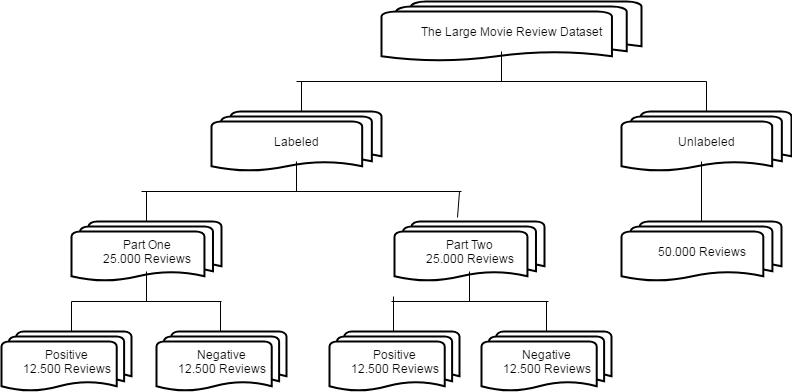
\includegraphics[width=5in, height=3in]{dataset} 
\caption{The Large Movie Review Dataset.\label{Figure 1}}
\end{figure}

The reviews in the dataset are stored as text files, where each file has a unique ID and an associated rating within the title of the file. The file itself contains the review in raw text format, which means that the text in the file is exactly as the reviewer wrote it on the IMDb website. Because of this, there could be some noise since the reviewer might have misspelled words or made use of an unconventional way of punctuation. This has to be taken into account when evaluating the results of classification presented in this paper. 

\newpage

\subsection{Collection of movie-specific aspects}

To collect the movie-specific aspects, the IMDb 5000 Movie Dataset was used. This is a dataset that contains information about more than 5000 distinct movies, including their title, genre, director and top 3 actors. The aspects were gathered from this dataset and saved as lists in text-files to be used as feature vectors during the classification task. The IMDb 5000 Movie Dataset was gathered by using a Python scraping tool to scrape the IMDb website for the information. In the dataset there are 5043 movie titles, 2400 director names and thousands of actor names. Altogether, this dataset provides for quite an extensive collection of feature sets.

\section{Annotated dataset}

The Large Movie Review Dataset was compiled by \citet{maas2011learning} as an annotated dataset, which means that the reviews were gathered based on their ratings. As indicated in the introduction, ratings are used for the annotation of the dataset, where a rating of 4 or lower is considered negative and a rating of 7 or higher is considered positive. As a result, the dataset is polarized, only containing reviews that have either a convincing negative or a convincing positive rating. The binary polarized nature of the dataset makes it extremely suitable for binary classification purposes. The two parts of the dataset are divided evenly, with 12.500 positive reviews and 12.500 negative reviews each. In this experiment, one part of the dataset is used as the development set, where all the different features are tested for their predictive power. The second part of the dataset is used as a final testing set, for which the classification results are presented in this paper.

\section{Processing}

\subsection{Creation of the dataframe}

Since the reviews are all stored in raw text files, some pre-processing is needed before the classification task can be performed. The first step in the processing of the data is the creation of a pandas dataframe within Python. The created dataframe contains the text and the label of every review, with the unique ID of the file as the index. The second step is to perform feature extraction, where all the different aspects are extracted from the text of the movie reviews. The results are stored in the same dataframe mentioned above. 

To extract a feature from the text, a text file is used in which all the keywords for every feature set are stored. As an example, the file for the 'genre' feature set contains words like 'action', 'adventure' and 'horror'. On every new line in the text file, one of these words is stored. In Appendix 1, Figure \ref{Figure 3} the first few rows of the created dataframe can be seen. There is a column for every feature set, and in every row there is the information that is extracted per feature for a given movie review.

\subsection{Tokenization of text}

Once the dataframe containing the raw text and the features is created, a tokenization step is performed. In this step, the raw text is processed further by a vectorizer to extract the tokens from the text and remove punctuation. In scikit-learn, the countvectorizer is used to process the raw text into a document-term matrix within pandas, that can be used by the classifier to perform sentiment analysis. The countvectorizer tokenizes the text, removing punctuation and keeping track of all occurrences of the different tokens in the reviews.

\chapter{Method}

As discussed in the second chapter, this research will compare general features to movie-specific aspects. The general features in this paper are \textit n-grams and a sentiment lexicon. The movie-specific aspects are actors, directors, genre and movie titles. The investigation is divided into two parts: classification and feature analysis. In the classification part of the research all the different feature sets will be tested and the results evaluated. In the feature analysis part, an in-depth look into the movie-specific aspects will be given to study exactly why the several aspects perform in their specific manner. 

This paper attempts to perform the classification based on frequencies of movie-aspects, rather than opinions expressed about these aspects. By counting occurrences of aspects such as actor names or mentions of genre, I can determine whether the mention of a certain actor or genre is an indication of that review being either positive or negative. 

The results of this research will provide new insights into how movie-specific aspects can be used to perform sentiment classification on movie reviews. Combining the results of this investigation with previous investigations that use parsing and semantic structures, a new and better baseline can be provided for performing similar classification tasks on movie reviews.

\section{Feature selection}

As mentioned in the previous chapter, the movie-specific aspects are all extracted from the IMDb 5000 Movie Dataset. There is a small overlap between the list of actors and the list of directors, since some actors of movies were also directors for other movies in the dataset. For this reason, these two feature sets were made mutually exclusive to make the classification results easier to interpret. For every person that was mentioned in both the actors and the directors feature set, he or she was removed from the directors list. I decided to treat the data in this way since it is more common for an actor to start directing at some point in his career than the other way around. Thus, I made the naive assumption that people that appear in both lists are more likely to be an actor first and a director second. To give a short overview, these are all the feature sets that will be evaluated during this investigation: 

\begin{enumerate}
\item{General features};
\begin{enumerate}
\item \textit N-grams (the text in the review);
\item Sentiment words (polarized words that indicate a certain sentiment).
\end{enumerate}
\item{Movie-specific features}
\begin{enumerate}
\item Actors (names of actors that are mentioned in the review);
\item Directors (names of directors that are mentioned in the review);
\item Genre (mentions of genre in the review);
\item Movie titles (mentions of movie titles in the review).
\end{enumerate}
\end{enumerate}

\newpage

Concerning the movie-specific features, I only use movie titles, genres and names of actors and directors that are explicitly mentioned in the review. Besides this, no other linguistic expressions are considered in the experiment. This means that if a reviewer writes about 'the lead actor' for instance, without mentioning his or her name explicitly, this information is not considered by the classifier. Also, sentiment expressed about any of the movie-specific aspects is not considered by the classification performed. These things need to be considered when interpreting the results presented in the next chapter.

\section{Classification}

The general and movie-specific feature sets will first be tested separately. After this, the movie-specific feature sets will also be combined to investigate if this leads to an increase in performance. It might be the case that the movie-specific feature sets perform better when combined with each other than just on their own merits. 

Because this research also takes \textit n-grams into account, all the feature sets are tested three times. As discussed in the second chapter, unigrams, bigrams and trigrams are considered in this paper. For the classification algorithms, I also use two different types: the Naive Bayes and the Linear SVC. Thus, in total, I performed the classification experiment six times, with three different \textit n-grams and two different classifiers. Hence, I will not only examine which feature sets perform best compared to each other, but also which feature sets perform best when used in a certain classification algorithm. This provides a more complete overview of the performance of feature sets for movie reviews.

To visualize the classification process, a flow chart for the algorithm used to perform this task has been included below. As can be seen in Figure \ref{Figure 2} the algorithm takes a set of documents as its input. It then extracts the needed information (text and features) and performs classification on them with both a Naive Bayes and a Linear SVC algorithm. The accuracy, precision, recall and F1-scores are automatically computed and reported by the algorithm. After this, certain features can be combined and the classification will again be performed on these new combinations of feature sets.

\begin{figure}[hbtp]\centering
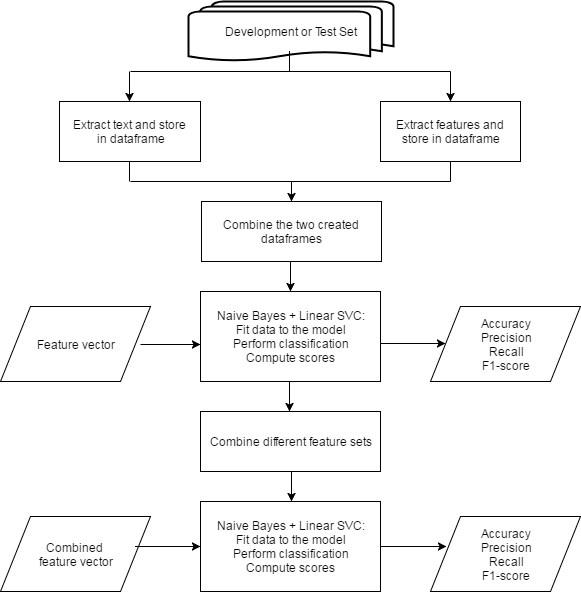
\includegraphics[width=4in, height=3in]{classification} 
\caption{Flow chart of the classification task.\label{Figure 2}}
\end{figure}

\section{Evaluation}

To determine how well the different feature sets perform I will analyze the results with the use of four different evaluation scores. The most intuitive of these scores is accuracy, which indicates how many of the predicted reviews are predicted to be the right class. This is possible due to the supervised learning nature of this experiment. The F1-score is another good measure of performance in classification, since this is the harmonic mean of precision and recall. The higher the accuracy and F1-scores are, the better a certain feature set performs when predicting the right class for the review.

The goal of the feature sets is to outperform the baseline, which is set at 50\% accuracy based on random guessing. Due to the fact that this is a binary classification experiment, where there are two possible outcomes (positive or negative), random guessing would yield an accuracy score of around 50\%. Furthermore, the dataset is divided evenly into positive and negative reviews.

\section{Feature analysis}

To provide for a deeper understanding of the results of movie-specific features, a more in-depth analysis will be done in this section of the investigation. To do this, all occurrences of the different aspects are counted in both the positive and negative reviews. Then, all mentions of unique actors, directors, genres and movie titles in positive and negative reviews can be closely studied. With this information, it is possible to provide better insights into the feature vectors that are used by the classifier to make predictions. An algorithm has been developed which can be seen in Appendix 1, Figure \ref{Figure 4}.

One of the analysis steps is keeping track of the relative occurrences of a certain feature set. For some aspects there might be more overall occurrences in positive or negative reviews. To make proper comparisons between positive and negative reviews, the data will be normalized by computing their relative occurrences compared to the overall total. 

Secondly, excluding entities that appear in both positive and negative reviews can provide more insight. This way, lists of movie-specific aspects that appear exclusively in positive or negative reviews are obtained. This information might be useful in future classification tasks on movie reviews.

Lastly, a Chi-squared test of independence can be performed to test whether the class of a review is dependent on a certain movie-specific aspect. The Chi-squared test of independence tests the null hypotheses that two variables are independent of each other. Thus, when significance is reached, this means the review sentiment is dependent on the tested movie aspect. For mentions of movie titles I will only look at titles that are mentioned exclusively in either positive or negative reviews, so no Chi-squared test for independence will be done for this feature set.

The code that was used in this experiment can be found at \\
https://github.com/TomKosse1/Thesis.git. To have a better understanding of the scripts, two examples have been included in Appendix 4. In Figure \ref{Figure 5} an example of the classification code can be seen, and in Figure \ref{Figure 6} an example of the feature analysis code.

\chapter{Results and Discussion}

\section{Classification results}

The results for unigrams can be seen in Table~\ref{Table 1}. The tables for bigrams and trigrams can be found in Appendix 2, Table~\ref{Table 4} and \ref{Table 5}. The trigrams performed worse compared to the unigrams and bigrams, so will therefore not be discussed here.

\subsection{Train-test splits}

During the development phase of the investigation different train-test split parameters have been tested to see what percentage of training versus testing data performed best overall. In most cases, a situation where 90\% of the data is used for training and 10\% of the data is used for testing is ideal. Therefore, all the results provided in this chapter were produced under this train-test ratio.

\subsection{Unigram results}

\begin{table}[hbtp]
\centering
\caption{Unigrams}
\label{Table 1}
\begin{tabular}{@{}lllll@{}}
\toprule
Naive Bayes Features                          & Accuracy & Precision & Recall & F1-score \\ \midrule
Text                              & 85.6\%       & 84.4\%          & 87.8\%       & 86.1\%         \\
Sentiment                         & 85.2\%         & 86.0\%          & 84.6\%       & 85.3\%         \\
Actors                            & 54.0\%         & 68.0\%          & 17.0\%       & 27.2\%         \\
Directors                         & 51.2\%         & 64.9\%          & 7.9\%       & 14.1\%         \\
Genre                             & 53.7\%         & 57.1\%          & 34.2\%       & 42.8\%         \\
Titles                            & 54.8\%         & 62.7\%          & 26.4\%       & 37.2\%         \\
Actors + Directors                        & 54.9\%         & 67.2\%          & 21.3\%       & 32.4\%         \\
Actors + Directors + Genre                        & 58.6\%         & 62.8\%          & 44.5\%       & 52.1\%         \\
Actors + Directors + Genre + Titles                       & 61.0\%         & 64.9\%          & 49.8\%       & 56.4\%          \\
Actors + Directors + Genre + Sentiment + Titles                    & 85.2\%          & 85.2\%          & 85.5\%       & 85.4\%         \\ 
\end{tabular}
\begin{tabular}{@{}lllll@{}}
\toprule
Linear SVC Features                          & Accuracy & Precision & Recall & F1-score \\ \midrule
Text                              & 89.1\%       & 89.4\%          & 89.1\%       & 89.2\%         \\
Sentiment                         & 82.9\%         & 83.4\%          & 82.8\%       & 83.1\%         \\
Actors                            & 58.4\%         & 55.3\%          & 92.5\%       & 69.2\%         \\
Directors                         & 54.6\%         & 52.8\%          & 97.0\%       & 68.4\%         \\
Genre                             & 55.4\%         & 54.9\%          & 67.0\%       & 60.3\%         \\
Titles                            & 56.9\%         & 55.4\%          & 75.8\%       & 64.0\%         \\
Actors + Directors                        & 60.3\%         & 56.7\%          & 91.1\%       & 69.9\%         \\
Actors + Directors + Genre                        & 62.4\%         & 60.0\%          & 77.4\%       & 67.6\%         \\
Actors + Directors + Genre + Titles                       & 63.2\%         & 61.6\%          & 72.8\%       & 66.7\%         \\
Actors + Directors + Genre + Sentiment + Titles                    & 82.8\%         & 83.8\%          & 82.0\%       & 82.9\%         \\ \bottomrule
\end{tabular}
\end{table}

As can be seen in Table~\ref{Table 1} containing the unigram results, some features outperform the baseline by a large margin. Overall, for nearly all features except the sentiment lexicon, the Linear SVC algorithm outperforms the Naive Bayes algorithm with a margin of about 2-5\%. The highest accuracy and F1-score comes from the 'text' feature performed by the Linear SVC algorithm. The sentiment lexicon is the only feature that performs better with the Naive Bayes classification, by a margin of about 2-3\%. This is a peculiar result since I would expect all features to perform better with the Linear SVC due to its robustness to noise, as mentioned previously.

The movie-specific features do not perform as well as expected. However, if all the movie-specific features are combined together the accuracy score is more than 13\% above the baseline. Each time another movie-specific feature set is added, the results become slightly better. Despite this, adding all the movie-specific feature sets to the sentiment feature set has a negative effect on the overall performance.

\subsection{Bigram results}

For the bigrams results in Table~\ref{Table 4}, the most noticeable is the high score for the 'text' feature in the Naive Bayes classification, which has close to 90\% accuracy and F1-score. This time, Naive Bayes outperforms the Linear SVC on this feature, and the feature also outperforms its unigram equivalent. This is also the highest accuracy and F1-score acquired during this investigation, closely followed by the unigram score for the 'text' feature in Linear SVC. 

For the movie-specific feature sets, combining them yields the best result once again. There is no significant improvement made with the bigrams compared to the unigrams (a margin of at most 3\%). Both the F1-score and accuracy score are fairly similar in unigrams and bigrams. As mentioned before, the sentiment lexicon seems to perform best when using Naive Bayes, while the other features perform better with the Linear SVC.

\section{Feature analysis}

\subsection{Sentiment words}

For the sentiment lexicon, there are more sentiment words in positive reviews (885.101) than negative reviews (866.802). In negative reviews, 34.7\% of sentiment words have a positive sentiment and 65.3\% have a negative sentiment. This makes sense, since I would expect  that a negative review contains more negative words. However, in positive reviews 45.8\% of sentiment words is positive and 54.2\% is negative. This is counter-intuitive, but the sentiment feature still performs fairly well. The sentiment feature would have performed even better if there were more positive words than negative words in the positive reviews.

Judging from Table~\ref{Table 1} and \ref{Table 4}, most movie-specific features perform up to 8\% above the baseline, for both Linear SVC and Naive Bayes. Before an in-depth analysis of movie-specific features is done, the average word count per review class is computed. A positive review has an average of 114 words per review, while a negative review has an average of 112 words per review. Thus, there are no significant differences in review length between positive and negative reviews.

\subsection{Actors and directors}

In the actors feature set, 67.8\% of actors are found in positive reviews, while 32.2\% are found in negative reviews. This indicates that reviewers mention actor names more in positive reviews. When actor occurrences are studied more closely, numerous actors that occur in positive reviews also occur in negative reviews, as can be seen in Appendix 3, Table~\ref{Table 6}. 

In the top 10 list of mentioned actors, a big overlap can be seen between the positive and negative reviews, where half of the actors occur in both review classes. In the relative columns, where occurrences are expressed in percentages compared to the total, there is a big difference between actors in positive reviews and the same actors in negative reviews. 'Al Pacino' for instance, occurs almost twice as many times in positive reviews than in negative reviews. This information could be useful in future research, but needs to be utilized by the classifier.

For the directors, similar results were found. These movie-specific feature sets both have the same problem, namely the overlap. Because of this, they lose their predictive power in a machine learning classification. The top 10 directors can be found in Appendix 3, Table~\ref{Table 7}. Also, two tables have been created in which actors and directors are mentioned exclusively in either positive or negative reviews. This information can be seen in Appendix 3, Table~\ref{Table 8} and \ref{Table 9}. This data could be useful in future experiments for classifying movie reviews. 

\subsection{Genre}

The analysis of the genre feature set can be seen in Appendix 3, Table~\ref{Table 10}. Out of the total number of occurrences of genre, 55.4\% were in positive reviews and 44.6\% were in negative reviews. It is important to note here that not all occurrences of a genre refer to the genre itself. However, in order to do a proper analysis the naive assumption has been made that every mention is a reference to a genre. As expected, a genre like 'horror' occurs comparably more often in negative reviews than positive reviews. Although, as with the other movie-specific feature sets, genres occur too many times in both positive and negative reviews to have significant predictive power when utilized by a classifier.

\subsection{Movie titles}

Movie titles also do not have the predictive power that was expected. However, something interesting can be seen when the list of titles that appear exclusively in either positive or negative reviews is considered. This list of movie titles can be seen in Table~\ref{Table 2}, where the corresponding IMDb-scores have also been included. Judging from the table, movie titles that are exclusively mentioned in positive reviews tend to have much higher IMDb-ratings than movie titles that are exclusively mentioned in negative reviews. More specifically, movie titles that appear in positive reviews have ratings of 6.7 and higher, while movie titles that appear in negative reviews have ratings of 5.5 and lower. The only exception to this is '20.000 leagues under the sea', which has a rating of 7.2. This could be valuable information in future research, if IMDb-ratings of mentioned movie titles are taken into account when performing the classification task.

\begin{center}
\begin{table}[hbtp]
\caption{Top 10 Titles}
\label{Table 2}
\begin{tabular}{llllll}
\toprule
Positive Titles        & IMDb-score & Negative Titles              &  IMDb-score \\ \midrule
The young Victoria          & 7.3        & Son of the mask                    & 2.2        \\
Best in show               & 7.5        & The omega code                    & 3.5        \\
Black snake moan            & 7.0        & Half past dead                    & 4.6        \\
Pitch perfect               & 7.2        & The grudge 2                      & 5.0        \\
Gentleman's agreement      & 7.4        & Soul survivors                    & 3.9        \\
Driving lessons             & 6.8        & Freddy got fingered                & 4.5        \\
Punch-drunk love            & 7.3        & Hanging up                         & 4.7        \\
Return to me                & 6.9        & 20,000 leagues under the sea      & 7.2        \\
Diamonds are forever        & 6.7        & Red Sonja                         & 5.0        \\
The sea inside              & 8.0        & Exit wounds                        & 5.5           \\ \bottomrule
\end{tabular}
\end{table}
\end{center}

\subsection{Chi-squared test of independence}

\paragraph{Actors and directors}

After performing the Chi-squared test of independence, I came to the conclusion that review sentiment is dependent on the overall number of actor occurrences. With Chi-squared (291.66) and a p-value of < 0.001, the class-actor dependency is found to be significant. For the directors, a similar result is found. With Chi-squared (92.63) and a p-value of < 0.001, the class-director dependency is also found to be significant. In Table~\ref{Table 3} above, a list of famous actors and directors can be seen. All the names in this table occur in both positive and negative reviews, and the significant dependencies have been bolded.

\begin{table}[]
\centering
\caption{Actors and directors in both classes}
\label{Table 3}
\begin{tabular}{llllll}
\toprule
Actor             & Positive & Negative & Director          & Positive & Negative \\ \midrule
\textbf{Clint Eastwood}    & 108      & 54       & Alfred Hitchcock  & 61       & 42       \\
\textbf{Meryl Streep}      & 90       & 37       & Mel Gibson        & 29       & 36       \\
Al Pacino         & 78       & 51       & Peter Jackson     & 25       & 30       \\
Tom Hanks         & 74       & 47       & George Lucas      & 28       & 24       \\
Michael Douglas   & 49       & 38       & Steven Spielberg  & 39       & 21       \\
\textbf{Brad Pitt}         & 74       & 34       & James Cameron     & 25       & 24       \\
Denzel Washington & 56       & 30       & Guy Ritchie       & 15       & 32       \\
\textbf{Sean Connery}      & 80       & 24       & \textbf{Danny Devito}      & 57       & 5        \\
\textbf{Will Smith}        & 52       & 25      & \textbf{Christopher Nolan} & 24       & 4       \\
Natalie Portman   & 43       & 21       & Michael Bay       & 9        & 17       \\ \bottomrule
\end{tabular}
\end{table}

As can be seen, there are more cases where review sentiment is dependent on an actor than a director. Some of the actors in the table come close to significance, as for example 'Denzel Washington'. With Chi-squared (3.24) and a p-value of 0.06, 'Denzel Washington' is almost significant enough to say that the review sentiment is dependent on mentions of him. Other cases, like 'Sean Connery' seem to be very potent indicators of sentiment of the review. With Chi-squared (14.98) and a p-value of < 0.001, 'Sean Connery' is extremely significant, indicating that the sentiment of the review is very dependent on the occurrence of his name. This shows that some actors are better indicators of review sentiment than others.

Most director names do not reach significance in the Chi-squared test of independence, indicating that review sentiment is less dependent on directors than actors.  Some directors, like 'Danny Devito' reach a very high level of significance. With Chi-squared (24.46) and a p-value of < 0.001, the review sentiment is very dependent on the occurrence of 'Danny Devito'. Most of the directors in the list however, do not come close to reaching significance. 'Guy Ritchie' is one of the closest ones with Chi-squared (2.51) and a p-value of 0.11, even though this is still far from significant. Overall, it can be concluded that actors are more indicative of a review sentiment than directors.

\paragraph{Genre}

The Chi-squared test also indicates an overall dependency of sentiment on the genre. With Chi-squared (351.82) and a p-value of < 0.001, the class-genre dependency is found to be significant. As an example, let us consider the 'horror' genre. As mentioned above, this genre seems to be a good indicator of the sentiment of the review. With Chi-squared (91.95) and a p-value of < 0.001, the review sentiment seems to be highly dependent on the 'horror' genre. As another example, the Chi-squared test is done for the 'action' genre. With Chi-squared (5.78) and a p-value of 0.01, the sentiment of the review is dependent on the 'action' genre as well. However, the review sentiment is less dependent on the 'action' genre than on the 'horror' genre, even though they are both significant. Overall, all the different genres reach significance in the Chi-squared test of independence, indicating they have high potential in predictive power.

\chapter{Conclusion}

The goal of this paper was to find out which features of a movie review text are the most relevant and informative for automatically predicting the sentiment expressed by the reviewer by means of the movie's rating system. The investigated general features are \textit n-grams and sentiment lexicon, the movie-specific features are mentions of actors, directors, genre and movie titles. 

Based on the studies by \citet{simonoff2000predicting} and \citet{eliashberg1997film}, I expected that the movie-specific aspects would perform fairly well in a classification experiment. These studies show that famous actors and actresses and the genre of a movie can be of great influence on the success of a film, which in turn has an effect on review sentiments. 

However, there is a significant difference in predictive power for general features and movie-specific features. Overall, the most informative features of movie review texts for the automatic prediction of the user's sentiment are the general features. They perform significantly better in the classification task than the movie-specific features. Nevertheless, there is much room for improvement when it comes to the movie-specific feature sets.

\section{Results}

\subsection{General features}

The highest accuracy score in the classification experiment overall was achieved with the 'text' feature using bigrams, namely 89.2\%. This result was closely followed by the same feature, but with unigrams (89.1\%). Compared to the sentiment lexicon, the 'text' feature performed better in all the tested conditions. The Naive Bayes algorithm outperforms the Linear SVC algorithm for the general feature sets, with the exception of unigrams. The sentiment lexicon seems to be better utilized by Naive Bayes than Linear SVC. Unigrams and bigrams both perform well with the general feature sets in general.

\subsection{Movie-specific features}

In all situations, the movie-specific features perform best when combined together. However, actor names have the best predictive power out of the four movie-specific feature sets, with the highest accuracy score being 58.4\% in both unigrams and bigrams. This score was achieved using the Linear SVC algorithm, which overall yields better results than the Naive Bayes algorithm when it comes to movie-specific features. The highest score that was attained from the movie-specific features was 63.2\%, when all four are combined using unigrams. In all tested conditions, the directors feature has the least amount of predictive power of the four.

\newpage

\subsection{Feature analysis}

After a closer examination of the movie-specific feature sets, I found that the lack of predictive power lies in the fact that a lot of the features occur in both positive and negative reviews. However, there were many differences in the number of occurrences and relative occurrences of the different unique features. After performing the Chi-squared test of independence, an overall dependency was found between the actors, directors and genre and the sentiment of the review. 

When examining the genres, I found that the review sentiment was dependent on all the unique genres. For actors, this was also the case for many of the unique actor names. However, review sentiment did not have many significant dependencies on unique director names. Thus, actors and genres have a high potential in predicting power when utilized correctly by the classification algorithm, according to the results of the Chi-squared test of independence.

\section{Previous research}

The results achieved in this study provides for a higher baseline than previous studies. \citet{turney2002thumbs} achieve an accuracy score of about 66\% on movie reviews using an unsupervised learning model. In the study by \citet{pouransari2014deep}, 84\% accuracy is achieved by using a decision tree and bag-of-words model for sentiment analysis. \citet{chaovalit2005movie} achieve an accuracy score of almost 85\% using a supervised machine learning model with movie reviews. In this paper, an accuracy score of almost 90\% is acquired on movie reviews, which is a substantial improvement.

There are no studies that have used frequencies of unique actor and director names or mentions of genre and movie titles as features. However, a similar study has been done for product aspects. In the paper by \citet{yu2011aspect}, discussed in the introduction, the authors obtain accuracy scores between 70\% and 90\%, which is higher than this investigation achieved. However, as stated in the introduction, aspects of products are usually better defined which leads to reviewers expressing sentiment on the same aspects much more frequently. 

\section{Future work}

In future work, if relative occurrence is taken into account by the classifier for the actors, directors and genre feature sets, significant improvement on predictive power should be achieved. This is confirmed by the Chi-squared test of independence, which also indicates that genre and actors should have more predictive power than directors. For the movie titles, the IMDb-rating could be taken into account by the classifier, which should improve the predictive power of this feature set as well. 

As mentioned in the second chapter there are also some limitations to the research done in this paper. Namely, linguistic expressions and sentiment expressed on the movie-specific features are not considered by the classifier. However, if this information would be used in conjunction with the potential improvements mentioned above, a significant increase in predictive power could be realized when using movie-specific aspects as features for classification of movie reviews.

%----------------------------------------------------------------------------------------
%	BIBLIOGRAPHY
%----------------------------------------------------------------------------------------

\cleardoublepage
\addcontentsline{toc}{chapter}{Bibliography}
\bibliographystyle{chicago} 
\bibliography{thesis-IK}

\chapter*{Appendix 1}
\markboth{Appendix 1}{Appendix 1}
\addcontentsline{toc}{chapter}{Appendix 1}

\begin{figure}[hbtp]\centering
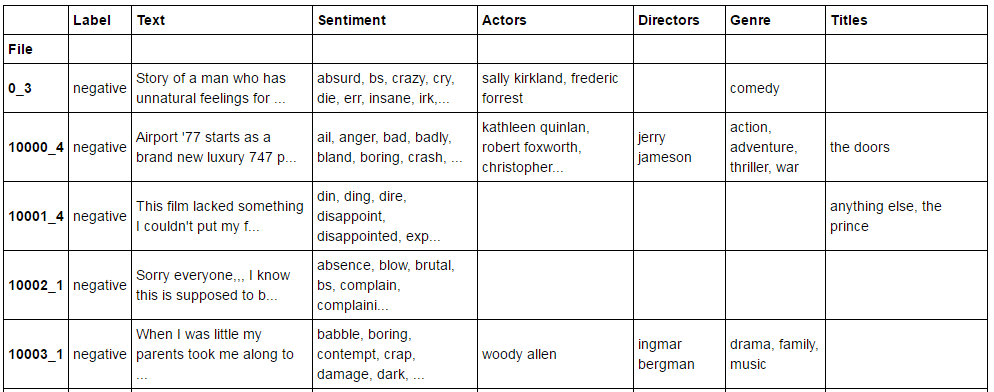
\includegraphics[width=5in]{dataframe} 
\caption{An extract from the pandas dataframe.\label{Figure 3}}
\end{figure}

\begin{figure}[hbtp]\centering
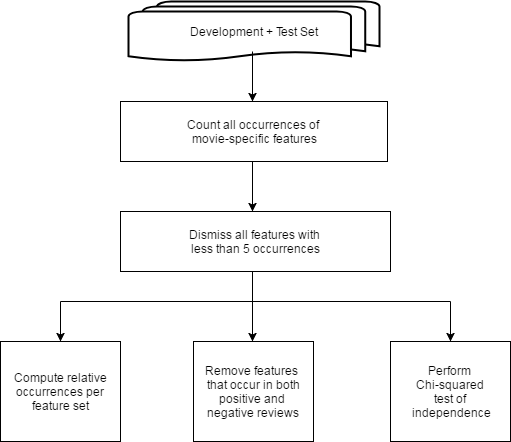
\includegraphics[width=4in, height=3in]{analysis} 
\caption{Flow chart of the feature analysis.\label{Figure 4}}
\end{figure}

\chapter*{Appendix 2}
\markboth{Appendix 2}{Appendix 2}
\addcontentsline{toc}{chapter}{Appendix 2}

\begin{table}[hbtp]
\centering
\caption{Bigrams}
\label{Table 4}
\begin{tabular}{@{}lllll@{}}
\toprule
Naive Bayes Features                           & Accuracy & Precision & Recall & F1-score \\ \midrule
Text                              & 89.2\%       & 88.8\%          & 90.0\%       & 89.4\%         \\
Sentiment                         & 83.2\%         & 84.1\%          & 82.4\%       & 83.2\%         \\
Actors                            & 54.6\%         & 72.3\%          & 16.5\%       & 26.9\%         \\
Directors                         & 51.2\%         & 66.7\%          & 7.3\%       & 13.1\%         \\
Genre                             & 51.2\%         & 57.3\%          & 14.0\%       & 22.5\%         \\
Titles                            & 53.7\%         & 59.8\%          & 26.1\%       & 36.3\%         \\
Actors + Directors                        & 56.0\%         & 71.9\%          & 21.4\%       & 33.0\%         \\
Actors + Directors + Genre                        & 57.4\%         & 68.5\%          & 29.2\%       & 41.0\%         \\
Actors + Directors + Genre + Titles                       & 61.1\%         & 68.3\%          & 43.1\%       & 52.8\%         \\
Actors + Directors + Genre + Sentiment + Titles                    & 83.9\%         & 84.8\%          & 83.2\%       & 84.0\%         \\
\end{tabular}
\begin{tabular}{@{}lllll@{}}
\toprule
Linear SVC Features                           & Accuracy & Precision & Recall & F1-score \\ \midrule
Text                              & 87.9\%       & 89.4\%          & 86.3\%       & 87.9\%         \\
Sentiment                         & 80.0\%         & 82.2\%          & 77.1\%       & 79.6\%         \\
Actors                            & 58.4\%         & 55.3\%          & 93.3\%       & 69.4\%         \\
Directors                         & 54.5\%         & 52.7\%          & 97.1\%       & 68.4\%         \\
Genre                             & 54.2\%         & 53.1\%          & 81.5\%       & 64.3\%         \\
Titles                            & 56.4\%         & 55.0\%          & 76.0\%       & 63.8\%         \\
Actors + Directors                        & 60.4\%         & 56.7\%          & 92.0\%       & 70.2\%         \\
Actors + Directors + Genre                        & 61.2\%         & 58.3\%          & 81.8\%       & 68.1\%         \\
Actors + Directors + Genre + Titles                       & 63.0\%         & 60.8\%          & 76.0\%       & 67.6\%         \\
Actors + Directors + Genre + Sentiment + Titles                    & 81.2\%         & 82.4\%          & 80.1\%       & 81.2\%         \\ \bottomrule
\end{tabular}
\end{table}

\begin{table}[hbtp]
\centering
\caption{Trigrams}
\label{Table 5}
\begin{tabular}{@{}lllll@{}}
\toprule
Naive Bayes Features                           & Accuracy & Precision & Recall & F1-score \\ \midrule
Text                              & 88.4\%       & 87.0\%          & 90.5\%       & 88.7\%         \\
Sentiment                         & 78.4\%         & 80.1\%          & 76.2\%       & 78.1\%         \\
Actors                            & 50.5\%         & 75.9\%          & 3.2\%       & 6.2\%         \\
Directors                         & 49.5\%         & 60.0\%          & 0.5\%       & 0.9\%         \\
Genre                             & 49.4\%         & 50.0\%          & 6.3\%       & 11.2\%         \\
Titles                            & 51.1\%         & 57.9\%          & 12.4\%       & 20.4\%         \\
Actors + Directors                        & 51.1\%         & 76.9\%          & 4.7\%       & 8.9\%         \\
Actors + Directors + Genre                        & 53.0\%         & 68.3\%          & 13.4\%       & 22.5\%         \\
Actors + Directors + Genre + Titles                       & 55.7\%         & 64.5\%          & 27.8\%       & 38.9\%         \\
Actors + Directors + Genre + Sentiment + Titles                    & 79.2\%         & 80.7\%          & 77.2\%       & 78.9\%         \\ 
\end{tabular}
\begin{tabular}{@{}lllll@{}}
\toprule
Linear SVC Features                           & Accuracy & Precision & Recall & F1-score \\ \midrule
Text                              & 83.6\%       & 86.6\%          & 80.0\%       & 83.2\%         \\
Sentiment                         & 75.4\%         & 75.7\%          & 75.7\%       & 75.7\%         \\
Actors                            & 53.8\%         & 52.3\%          & 99.2\%       & 68.5\%         \\
Directors                         & 51.1\%         & 50.8\%          & 99.8\%       & 67.4\%         \\
Genre                             & 52.4\%         & 51.7\%          & 92.5\%       & 66.3\%         \\
Titles                            & 53.2\%         & 52.2\%          & 89.4\%       & 65.9\%         \\
Actors + Directors                        & 55.0\%         & 52.9\%          & 98.9\%       & 69.0\%         \\
Actors + Directors + Genre                        & 57.3\%         & 54.7\%          & 91.1\%       & 68.3\%         \\
Actors + Directors + Genre + Titles                       & 58.2\%         & 56.0\%          & 80.9\%       & 66.2\%         \\
Actors + Directors + Genre + Sentiment + Titles                    & 76.2\%         & 76.4\%          & 76.8\%       & 76.6\%         \\ \bottomrule
\end{tabular}
\end{table}

\chapter*{Appendix 3}
\markboth{Appendix 3}{Appendix 3}
\addcontentsline{toc}{chapter}{Appendix 3}

\begin{table}[hbtp]
\centering
\caption{Top 10 Actors}
\label{Table 6}
\begin{tabular}{@{}llllll@{}}
\toprule
Positive Actors & Absolute & Relative & Negative Actors & Absolute & Relative \\ \midrule
Clint Eastwood  & 108        & 0.59       & Woody Allen     & 79         & 0.43       \\
Meryl Streep    & 90         & 0,49      & Robin Williams  & 58         & 0.32       \\
Sean Connery    & 80         & 0.44       & Kevin Spacey    & 55         & 0.3       \\
Al Pacino       & 78         & 0.43        & Clint Eastwood  & 54         & 0.3       \\
Tom Hanks       & 74         & 0.41       & Morgan Freeman  & 53         & 0.29       \\
Brad Pitt       & 74         & 0.41       & Adam Sandler    & 53         & 0.29       \\
Robin Williams  & 60         & 0.33       & Christopher Lee & 52         & 0.29       \\
Bruce Willis    & 60         & 0.33       & Al Pacino       & 51         & 0.28       \\
Morgan Freeman  & 59         & 0.32        & Bruce Willis    & 49         & 0.27       \\ 
Rock Hudson  & 58         & 0.32        & Tom Hanks    & 47         & 0.26       \\ \bottomrule
\end{tabular}
\end{table}

\begin{table}[hbtp]
\centering
\caption{Top 10 Directors}
\label{Table 7}
\begin{tabular}{llllll}
\toprule
Positive Directors & Absolute & Relative & Negative Directors                                    & Absolute & Relative \\ \midrule
David Lynch        & 80       & 1.23     & Uwe Boll                                              & 87       & 1.34     \\
John Ford          & 79       & 1.21     & David Lynch                                           & 81       & 1.24     \\
Dustin Hoffman     & 69       & 1.06     & Steven Seagal                                         & 78       & 1.2      \\
John Carpenter     & 62       & 0.95     & Dennis Hopper                                         & 50       & 0.77     \\
Orson Welles       & 62       & 0.95     & Wes Craven                                            & 46       & 0.71     \\
Alfred Hitchcock   & 61       & 0.94     & Alfred Hitchcock                                      & 42       & 0.64     \\
Dennis Hopper      & 58       & 0.89     & Tim Burton                                            & 42       & 0.64     \\
Sean Penn          & 57       & 0.87     & John Carpenter                                        & 42       & 0.64     \\
Danny Devito       & 57       & 0.87     & Matt Dillon                                           & 40       & 0.61     \\
William H. Macy    & 56       & 0.86     & Ben Affleck								& 38       & 0.58    \\ \bottomrule
\end{tabular}
\end{table}

\begin{table}[hbtp]
\centering
\caption{Top 10 Exclusive Actors}
\label{Table 8}
\begin{tabular}{llllll}
\toprule
Positive Actors  & Absolute & Relative & Negative Actors       & Absolute & Relative \\ \midrule
Victor Mclaglen  & 38       & 0.21     & Jessica Simpson       & 29       & 0.16     \\
Jeremy Northam   & 35       & 0.19     & Joe Don Baker         & 28       & 0.15     \\
Emily Watson     & 32       & 0.18     & Mira Sorvino          & 22       & 0.12     \\
Jean Peters      & 30       & 0.16     & Faye Dunaway          & 21       & 0.12     \\
Ray Charles      & 28       & 0.15     & Sarah Michelle Gellar & 21       & 0.12     \\
Leslie Caron     & 28       & 0.15     & Anne Heche            & 20       & 0.11     \\
Robert Blake     & 28       & 0.15     & Rosanna Arquette      & 20       & 0.11     \\
Eleanor Parker   & 27       & 0.15     & Telly Savalas         & 19       & 0.1     \\
Ralph Richardson & 26       & 0.14     & Steve Guttenberg      & 18       & 0.1     \\
Sam Waterston    & 25       & 0.14     & Melanie Griffith      & 18       & 0.1     \\ \bottomrule
\end{tabular}
\end{table}

\begin{table}[]
\centering
\caption{Top 10 Exclsusive Directors}
\label{Table 9}
\begin{tabular}{llllll}
\toprule
Positive Directors   & Absolute & Relative & Negative Directors & Absolute & Relative \\ \midrule
Terry Gilliam        & 31       & 0.48     & Uwe Boll           & 87       & 1.34     \\
Hayao Miyazaki       & 27       & 0.41     & Andy Garcia        & 12       & 0.18     \\
Christopher Nolan    & 24       & 0.37     & George A. Romero   & 12       & 0.18     \\
Lars Von Trier       & 22       & 0.34     & Richard Donner     & 10       & 0.15     \\
Elia Kazan           & 22       & 0.34     & Ruggero Deodato    & 10       & 0.15     \\
Michael Curtiz       & 21       & 0.32     & J. Lee Thompson    & 10       & 0.15     \\
Paul Thomas Anderson & 21       & 0.32     & Richard Kelly      & 10       & 0.15     \\
Richard Benjamin     & 21       & 0.32     & Michael Crichton   & 9        & 0.14     \\
Mike Judge           & 20       & 0.31     & Edward Burns       & 9        & 0.14     \\
Anthony Minghella    & 19       & 0.29     & Martin Lawrence    & 8        & 0.12    \\ \bottomrule
\end{tabular}
\end{table}

\begin{table}[hbtp]
\centering
\caption{Top 10 Genres}
\label{Table 10}
\begin{tabular}{@{}llllll@{}}
\toprule
Positive Genre & Absolute & Relative & Negative Genre & Absolute & Relative \\ \midrule
War            & 6956       & 11.69       & War            & 5971       & 10.03        \\
Music          & 3471       & 5.83       & Action         & 3105       & 5.22        \\
Action         & 3381       & 5.68       & Horror         & 2649       & 4.45        \\
Comedy         & 2583       & 4.34        & Music          & 2384       & 4.01        \\
Drama          & 2543       & 4.27        & Comedy         & 2154       & 3.62        \\
Family         & 2524       & 4.24        & Drama          & 1749       & 2.94         \\
Horror         & 1752       & 2.94        & Family         & 1527       & 2.57        \\
History        & 1274       & 2.14        & History        & 882        & 1.48        \\
Musical        & 893        & 1.5        & Thriller       & 732        & 1.23        \\
Thriller       & 874        & 1.47        & Mystery        & 629        & 1.06       \\ \bottomrule
\end{tabular}
\end{table}

\chapter*{Appendix 4}
\markboth{Appendix 4}{Appendix 4}
\addcontentsline{toc}{chapter}{Appendix 4}

\begin{figure}[hbtp]\centering
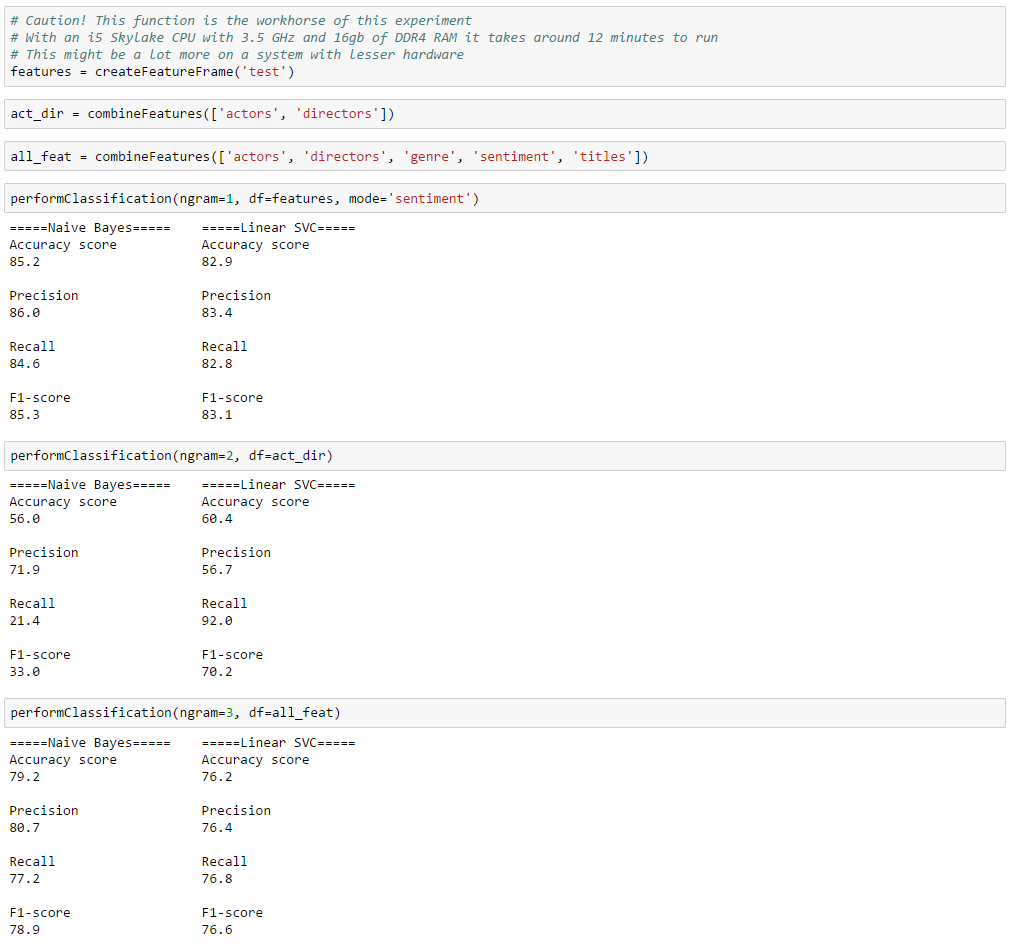
\includegraphics[width=6in, height=7in]{example_clf} 
\caption{Example use of classification code.\label{Figure 5}}
\end{figure}

\begin{figure}[hbtp]\centering
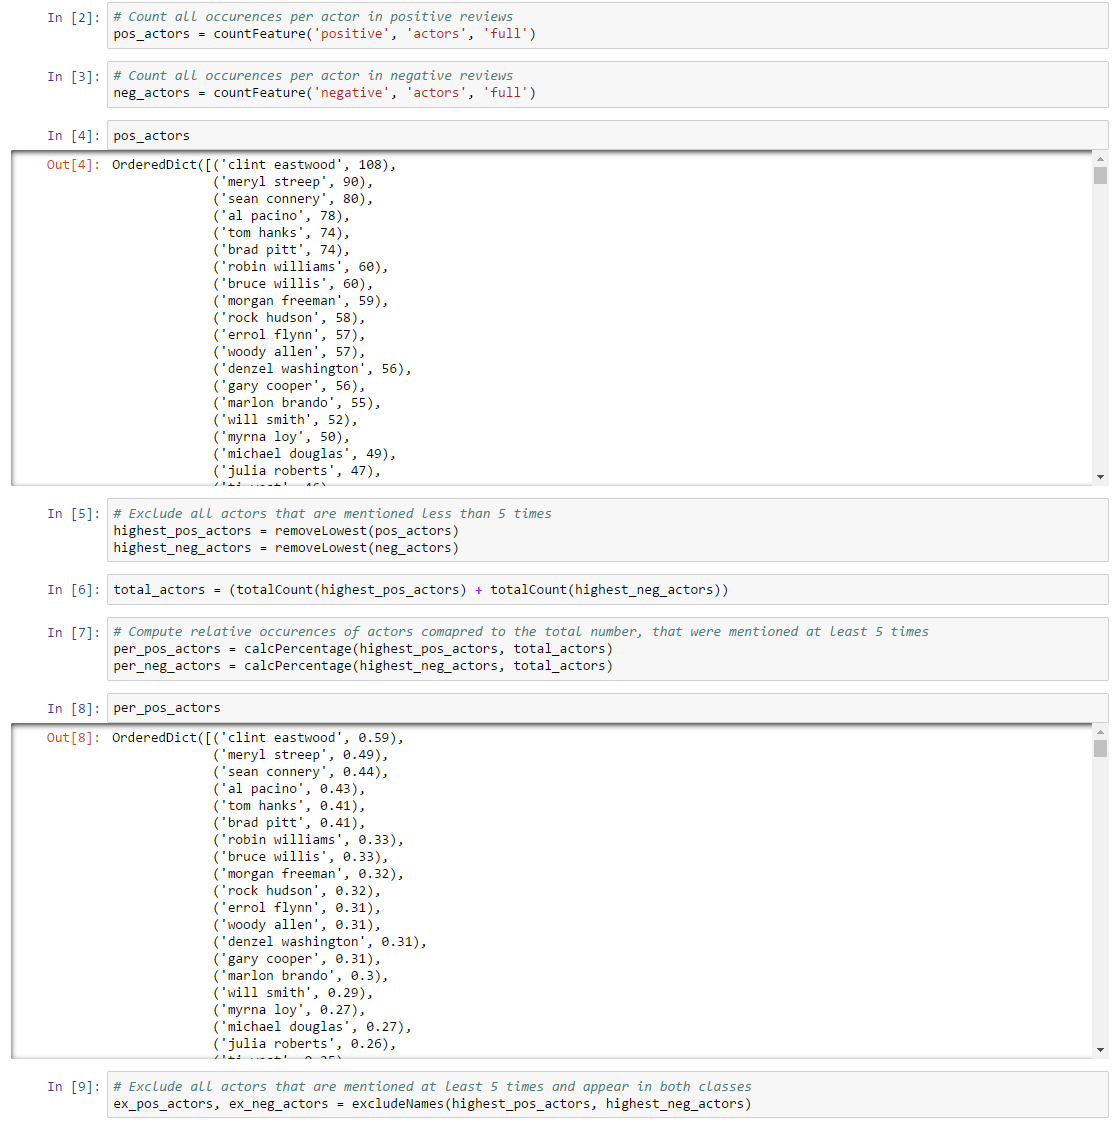
\includegraphics[width=6in, height=8in]{example_ana} 
\caption{Example use of feature analysis code.\label{Figure 6}}
\end{figure}

\end{document}